\documentclass{standalone}
\usepackage{tikz}
\usepackage{pgfplots}
\pgfplotsset{compat=1.18}

\begin{document}
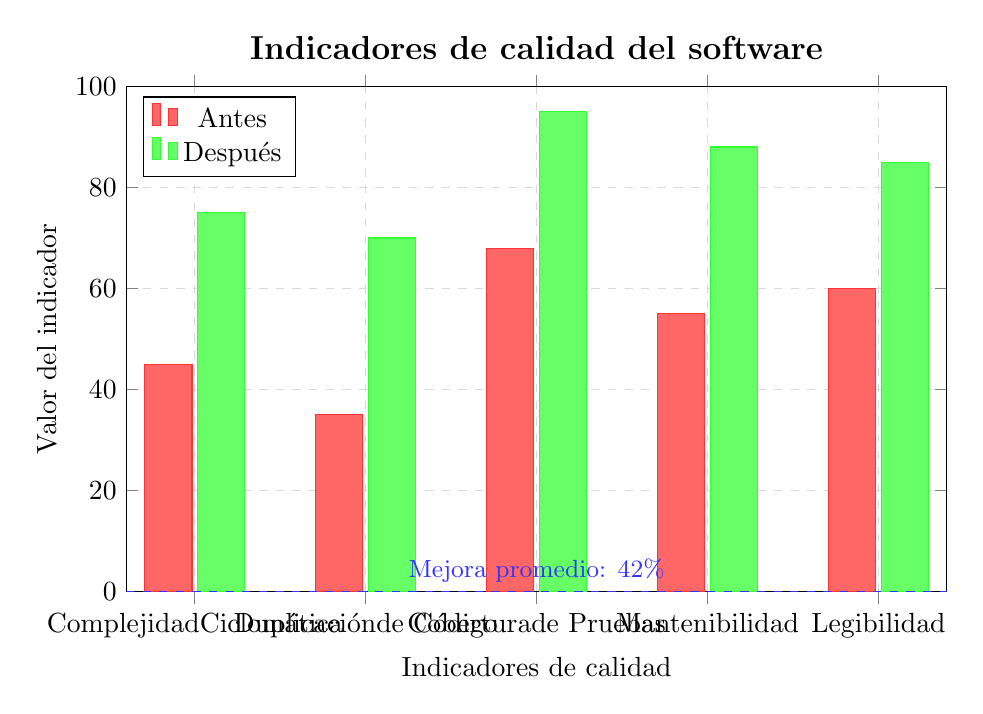
\begin{tikzpicture}
\begin{axis}[
    ybar,
    bar width=0.6cm,
    width=12cm,
    height=8cm,
    ylabel={Valor del indicador},
    xlabel={Indicadores de calidad},
    xtick=data,
    xticklabels={Complejidad\\Ciclomática, Duplicación\\de Código, Cobertura\\de Pruebas, Mantenibilidad, Legibilidad},
    ymin=0,
    ymax=100,
    grid=major,
    grid style={dashed,gray!30},
    legend pos=north west,
    legend style={at={(0.02,0.98)},anchor=north west},
    title={Indicadores de calidad del software},
    title style={font=\large\bfseries}
]

% Antes de implementar prácticas
\addplot[fill=red!60, draw=red!80] coordinates {
    (1, 45) (2, 35) (3, 68) (4, 55) (5, 60)
};

% Después de implementar prácticas
\addplot[fill=green!60, draw=green!80] coordinates {
    (1, 75) (2, 70) (3, 95) (4, 88) (5, 85)
};

\legend{Antes, Después}

% Agregar líneas de mejora
\draw[thick, blue!80, dashed] (axis cs:0.5, 0) -- (axis cs:5.5, 0);
\node[above, blue!80, font=\small] at (axis cs:3, 0) {Mejora promedio: 42\%};

\end{axis}
\end{tikzpicture}
\end{document}
